 % arara: xelatex: {shell: true}
% arara: biber
% arara: xelatex: {shell: true}
% arara: xelatex: {shell: true}

% Podklad k cvičení v předmětu BI-DPR
% autor: Ondřej Guth (ondrej.guth@fit.cvut.cz)
% (c) FIT ČVUT, 2018


\documentclass[a4paper]{article}
\usepackage{polyglossia}
\setmainlanguage{czech}
\usepackage{xevlna,xltxtra}
\usepackage{csquotes}
%\usepackage[style=german]{csquotes} % pro starší verze, kde není čeština

\usepackage[hidelinks]{hyperref}
\usepackage{graphicx}
\usepackage{minted}
\usepackage{xfrac}
\usepackage{nicefrac}
\usepackage[style=iso-numeric]{biblatex}

\title{MI-PAA\\
\large Úkol 4 -- zpráva\\}

\author{Tomáš Přeučil}

\begin{document}

\maketitle

%\tableofcontents

\section{Zadání úlohy}
	Zadáním úlohy byl výběr a naprogramování pokročilé heuristiky pro řešení problémů, jejichž konfigurační proměnnou je bitový vektor a testování na problému batohu. Na výběr byly tři možnosti: simulované ochlazování, genetický algoritmus a tabu prohledávání.
	
	Zvolena byla varianta s genetickým algoritmem.


\section{Použité prostředky}
	\subsection{Programovací jazyky a software}
		Úloha byla řešena v jazyce Python ve verzi 3.6 pod operačním systémem OS X 10.11.6. Program byl spouštěn z Bashe a tudíž pro spuštění nebylo využito žádné IDE.
		Pro měření času byla využita knihovna time a funkce \textit{time.process\_time()}. Jedná se o novinku od verze 3.3, která pracuje velmi podobně jako doporučovaná knihovna \textit{timeit}.
		
	\subsection{Konfigurace testovacího stroje}
		Testování bylo provedeno na MacBooku Pro 13", Early 2011, modelové číslo MC700LL/A. Stroj obsahuje CPU Intel Core i5 2415M (2,3~GHz) a 16~GB RAM. Jediný další rozdíl oproti výchozí konfiguraci je vyměněný disk (za SSD), což však v tomto případě nehraje roli.

\section{Rozbor algoritmu}
	Genetický algoritmus funguje tak, že postupně šlechtí co nejlepší jedince -- v tomto případě bitové vektory.
	
	Na začátku je nutné vytvořit počáteční populaci. To je možné udělat buď náhodně, nebo jedince \enquote{seedovat} do té oblasti stavového prostoru, kde by se mohlo nacházet řešení -- u problému batohu například vkládat primárně cenné věci.
	
	Tato populace je dále šlechtěna. Jednak se dva jedinci mohou s určitou pravděpodobností křížit, ale také mohou mutovat. Po jednom cyklu šlechtění tedy máme generaci obsahující původní rodiče, mutanty a potomky. V tuto chvíli je nutné nechat přežít pouze nejschopnější jedince.
	
	Docílit toho je poměrně snadné -- pole jedinců je seřazeno dle jejich \enquote{fitness}, což je atribut značící jejich vhodnost pro další přežití (u problému batohu například suma cen všech vložených věcí), a pole zkrátit na délku danou uživatelem.
	
	Po té, co je vyšlechtěno x populací, je z té poslední vybrán nejlepší jedinec, který je řešením.
	

\section{Rámcový popis postupu řešení}
	Algoritmus byl implementován přesně dle postupu uvedeného v předchozí kapitole. Zde uvedu pouze určité implementační detaily.
	
	Pro uložení dat bylo použito pole objektů \textit{chromosome}. Toto pole má velikost danou velikostí populace. Každý objekt v sobě ukládá svou fitness, kapacitu batohu, velikost batohu a pole objektů \textit{item}. Objekt \textit{item} v sobě ukládá present bit (zda-li je přítomen v batohu, to simuluje klasickou konfigurační proměnnou -- bitový vektor), svoji váhu a cenu. 
	
	Objekt \textit{chromosome} dále implementuje metody inicializace, mutace, křížení (druhým parametrem je jiný chromosom) a výpočtu fitness. Tím je dosaženo maximálního zapouzdření a v případě použití heuristiky pro jiný problém stačí vyměnit fitness funkci a inicializační část konstruktoru. Návrh objektu \textit{chromosome} funguje s libovolným objektem mající atribut \textit{present}.
	
	Výše zmíněná inicializační část je sama o sobě velmi zajímavá. Pokud je konstruktor volán s příznakem \textit{init = 1}, je provedena inicializace bitového vektoru. Pro problém batohu byla nejdříve vyzkoušena varianta s náhodnou inicializací, která však byla výrazně pomalejší a nedávala moc přesné výsledky. Z tohoto důvodu je bitový vektor inicializován následovně:
	
	\begin{itemize}
		\item Vypočti průměrnou cenu věci v batohu
		\item Má daná věc nadprůměrnou cenu a je její hmotnost menší než 80 \% kapacity?
			\begin{itemize}
				\item Pokud ano, s 66 \% pravděpodobností nastav proměnnou tmp na 1.
				\item S 33 \% pravděpodobností nastav proměnnou tmp na 0
			\end{itemize}
		\item Hoď kostkou.
			\begin{itemize}
				\item Pokud je výsledek sudý, vlož objekt do batohu.
				\item Pokud je výsledek lichý a proměnná tmp je rovna 1, vlož objekt do batohu
				\item Jinak objekt do batohu nevkládej.
			\end{itemize}
	\end{itemize}
	
	Dále je prováděn typický genetický algoritmus. Po mnoha experimentech se jako nejlepší hodnoty parametrů pro instance s 30-40 objekty ukázaly jako nejvhodnější parametry tyto (detaily se nachází v další kapitole):
	\begin{itemize}
		\item Pravděpodobnost mutace -- 8 \%
		\item Pravděpodobnost křížení -- 70 \%
	\end{itemize}	
	
	Maximální počet generací bez zlepšení byl nastaven na 20. (Což na grafu \ref{avg-fitness} není pro přehlednost zohledněno.)
	
	Následný výstup byl zpracován pomocí awk a LibreOffice.
	
\section{Výběr parametrů}
	Veškeré experimenty popsané v této kapitole byly prováděny na množině padesáti instancí o čtyřiceti věcech. V grafech je vždy vynesen průměr hodnot za celou množinu. Jednotka času jsou sekundy.
	
	V prvním kroku byla provedena měření pro deset různých pravděpodobností křížení. Pravděpodobnost mutace byla v tomto kroku nastavena na fixních 7 \%. Z grafu \ref{err-krizeni} je jasně patrné, že při pravděpodobnosti 70 \% je průměrná relativní chyba nejmenší.
	
	\begin{figure}[h]\centering
		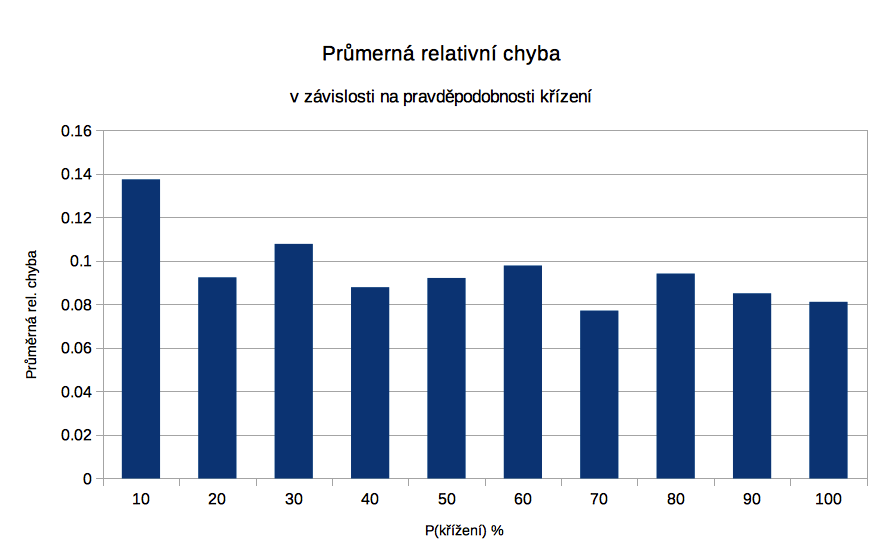
\includegraphics[width=0.99\textwidth]{chyba-krizeni.png} 
		\caption{Průměrná relativní chyba pro různé pravděpodobnosti křížení}
		\label{err-krizeni}
	\end{figure}
	
	V rámci tohoto měření byl kromě relativní chyby měřen i průměrný čas výpočtu. Lze říci, že pravděpodobnost křížení na něj nemá větší vliv. Měřené výsledky jsou na grafu \ref{time-krizeni}
	
	\begin{figure}[h]\centering
		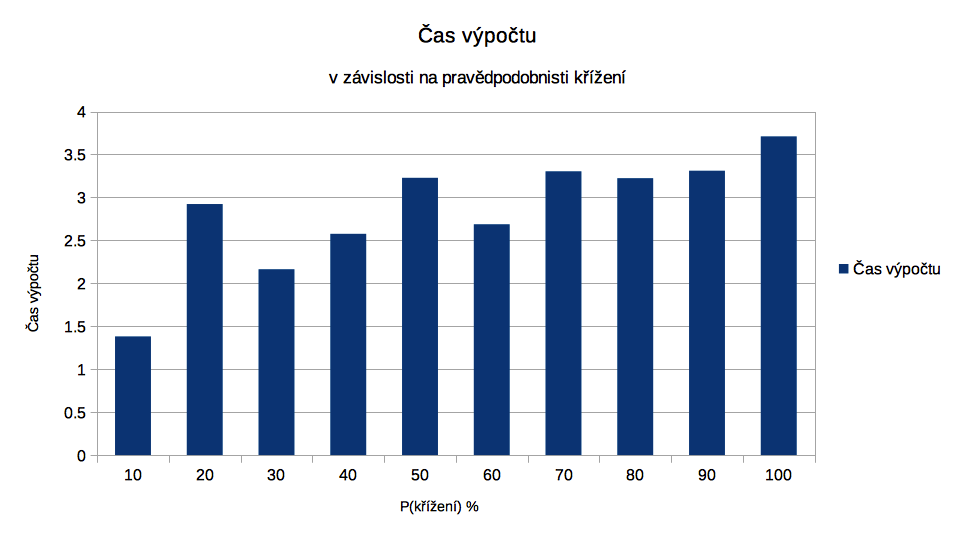
\includegraphics[width=0.99\textwidth]{cas-krizeni.png} 
		\caption{Průměrný čas výpočtu pro různé pravděpodobnosti křížení}
		\label{time-krizeni}
	\end{figure}
	
	Po zvolení P(křížení) = 70 \% byly provedeny testy pro pravděpodobnost mutace. Testované pravděpodobnosti byly od 0 \% do 19 \%.	 Z grafu \ref{err-mutace} lze vypozorovat, že relativní chyba klesá spolu se zvětšující se pravděpodobností. 
	
	\begin{figure}[h]\centering
		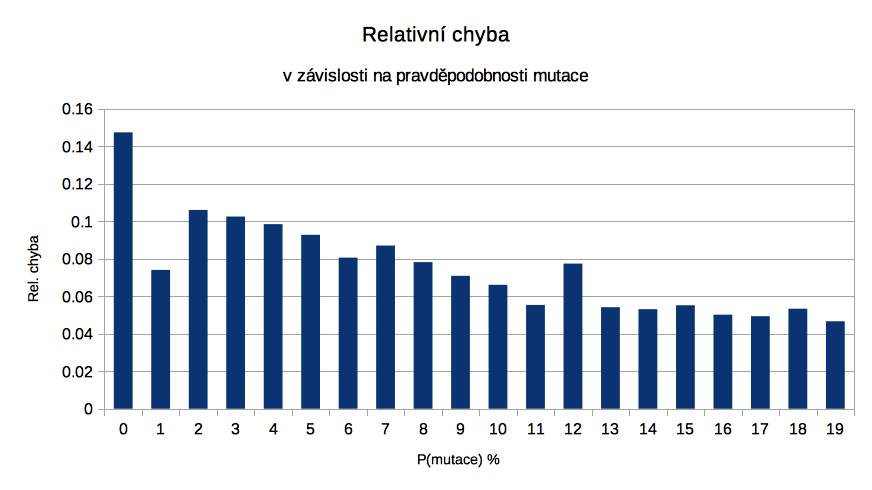
\includegraphics[width=0.99\textwidth]{chyba-mutace.png} 
		\caption{Průměrná relativní chyba pro různé pravděpodobnosti mutace}
		\label{err-mutace}
	\end{figure}
	
	Stejně jako v případě minulého měření byl i zde měřen průměrný čas výpočtu. Na rozdíl od pravděpodobnosti křížení má pravděpodobnost mutace výrazný vliv na čas výpočtu. Čím vyšší pravděpodobnost, tím delší výpočet.
	
	\begin{figure}[h]\centering
		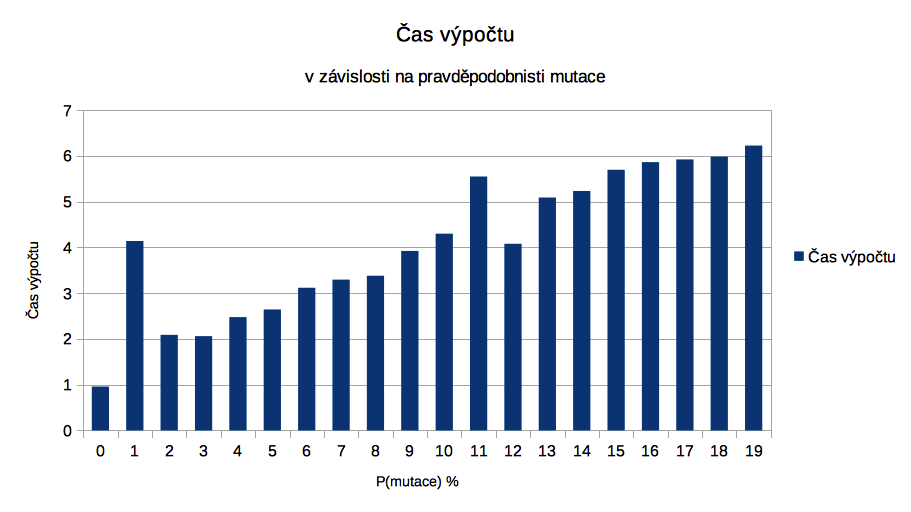
\includegraphics[width=0.99\textwidth]{cas-mutace.png} 
		\caption{Průměrný čas výpočtu pro různé pravděpodobnosti mutace}
		\label{time-mutace}
	\end{figure}
	
	Vzhledem k těmto pozorováním byl parametr P(mutace) zvolen v hodnotě 8 \%. Relativní chyba je zde necelých 8 \%, avšak čas výpočtu je ovlivněn v přijatelných mezích. Pro P(mutace) = 1 je doba výpočtu cca 2 s, pro P(mutace) = 15 téměř 6 s, avšak pro zvolený parametr 8 je průměrná doba výpočtu kolem 3,2 s.
	

\section{Naměřené výsledky}
	Veškerá měření byla prováděna na dodané sadě problémů o 40 věcech.
	
	Na grafu \ref{time} je znázorněn čas výpočtu pro jednotlivé instance problému. Průměrná doba výpočtu byla 3,2 s, což je výrazně více, než při dynamickém programování. Nejedná se však o nic nečekaného.
	
	\begin{figure}[h]\centering
		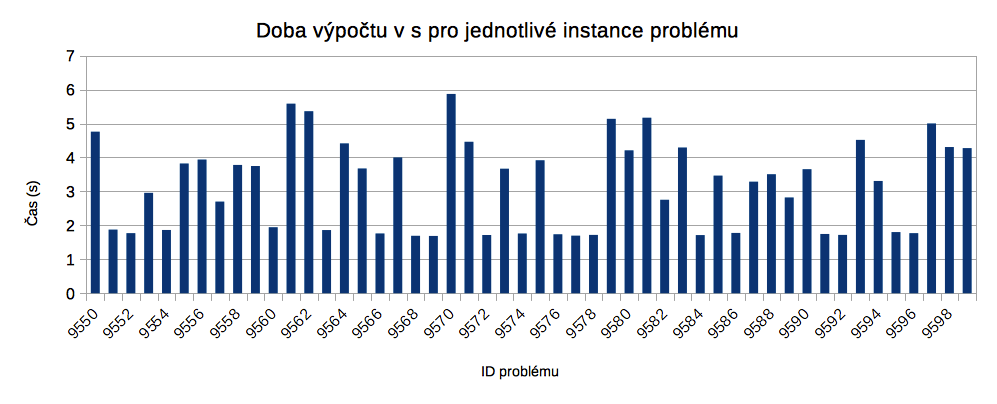
\includegraphics[width=0.99\textwidth]{doba-vypoctu.png} 
		\caption{Časy všech výpočtů}
		\label{time}
	\end{figure}
	
	Graf \ref{avg-fitness} znázorňuje průměrnou relativní fitness v průběhu generací. Zde byly naměřeny zdatnosti ve všech generacích u všech problémů a všechny instance byly pro danou generaci zprůměrovány. Referenčním maximem byla hodnota uvedená jako řešení v dodaném referenčním souboru. Důvodem pro vysokou počáteční fitness je způsob inicializace popsaný výše.

	\begin{figure}[h]\centering
		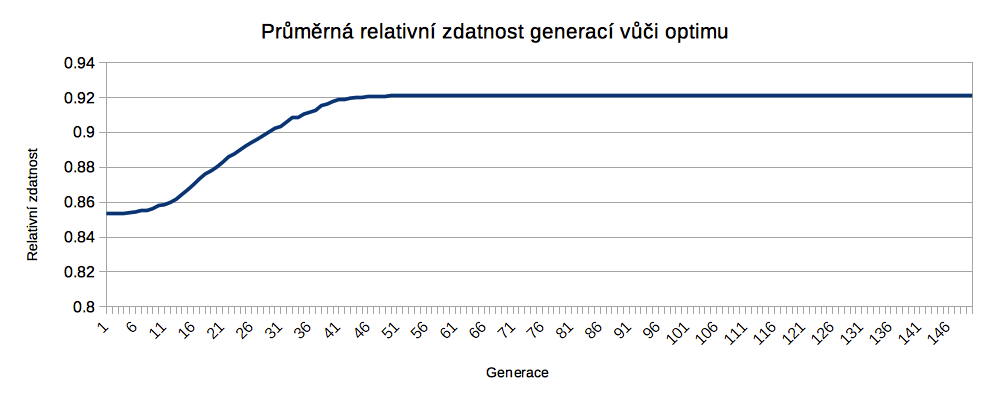
\includegraphics[width=0.99\textwidth]{prumerna-zdatnost.png} 
		\caption{Průměrná zdatnost dle generace}
		\label{avg-fitness}
	\end{figure}

	Poslední měřenou veličinou byla relativní chyba. Na grafu \ref{error} je znázorněna pro každou jednotlivou instanci problému. Průměr je 8,48 \%. Tento průměr se liší od hodnoty uvedené v minulé kapitole. Důvodem je to, že algoritmus není deterministický, z čehož plyne možná rozdílnost výsledků v různých bězích.
	
	\begin{figure}[h]\centering
		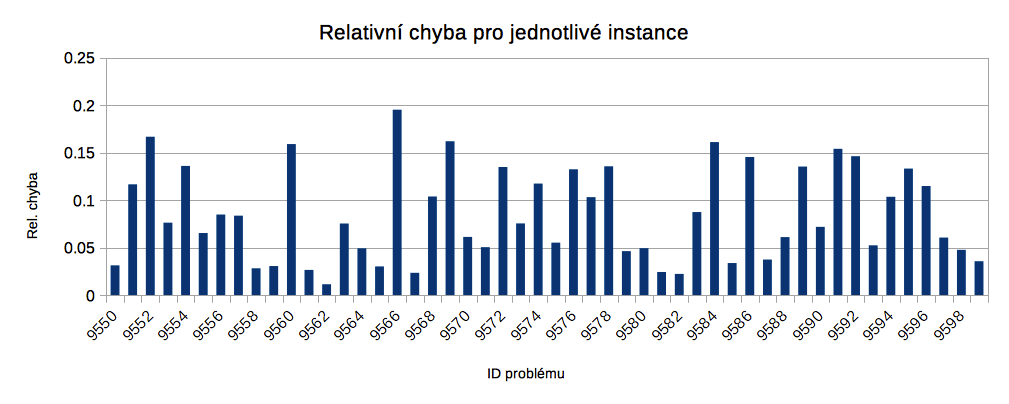
\includegraphics[width=0.99\textwidth]{rel-chyba.png} 
		\caption{Relativní chyba}
		\label{error}
	\end{figure}
	
	Nejlepší vyzkoušená nastavení parametrů jsou uvedena v předchozí kapitole. Co se počtu generací týče, cokoli pod 40 znamenalo velmi výrazné snížení výsledné fitness. Vzhledem k maximálně 20 průchodům bez zlepšení byl zvolen limit 150 generací.
	
	Nastavení maximální velikosti populace pod 250 značně zkreslilo výsledky. Nakonec byla zvolena hodnota 400.
	
\section{Závěr}
	Byla provedena implementace a analýza genetického algoritmu, který řeší problém batohu v průměrném čase 3,2 s a průměrnou relativní chybou 8,5 \%.
	
	Algoritmus se ukázal velmi pomalý oproti například dynamickému programování, na stranu druhou je mnohem univerzálnější a řeší libovolný problém, jehož konfigurační proměnnou je bitový vektor.
	
	Zároveň bylo pomocí objektového návrhu dosaženo vysoké míry zapouzdření a snadné přenositelnosti.

	V příloze se nachází naměřené výsledky ve formátu .ods, grafy v plném rozlišení a zdrojové kódy.


\end{document}